
\begin{figure*}[!tp]
    \centering
    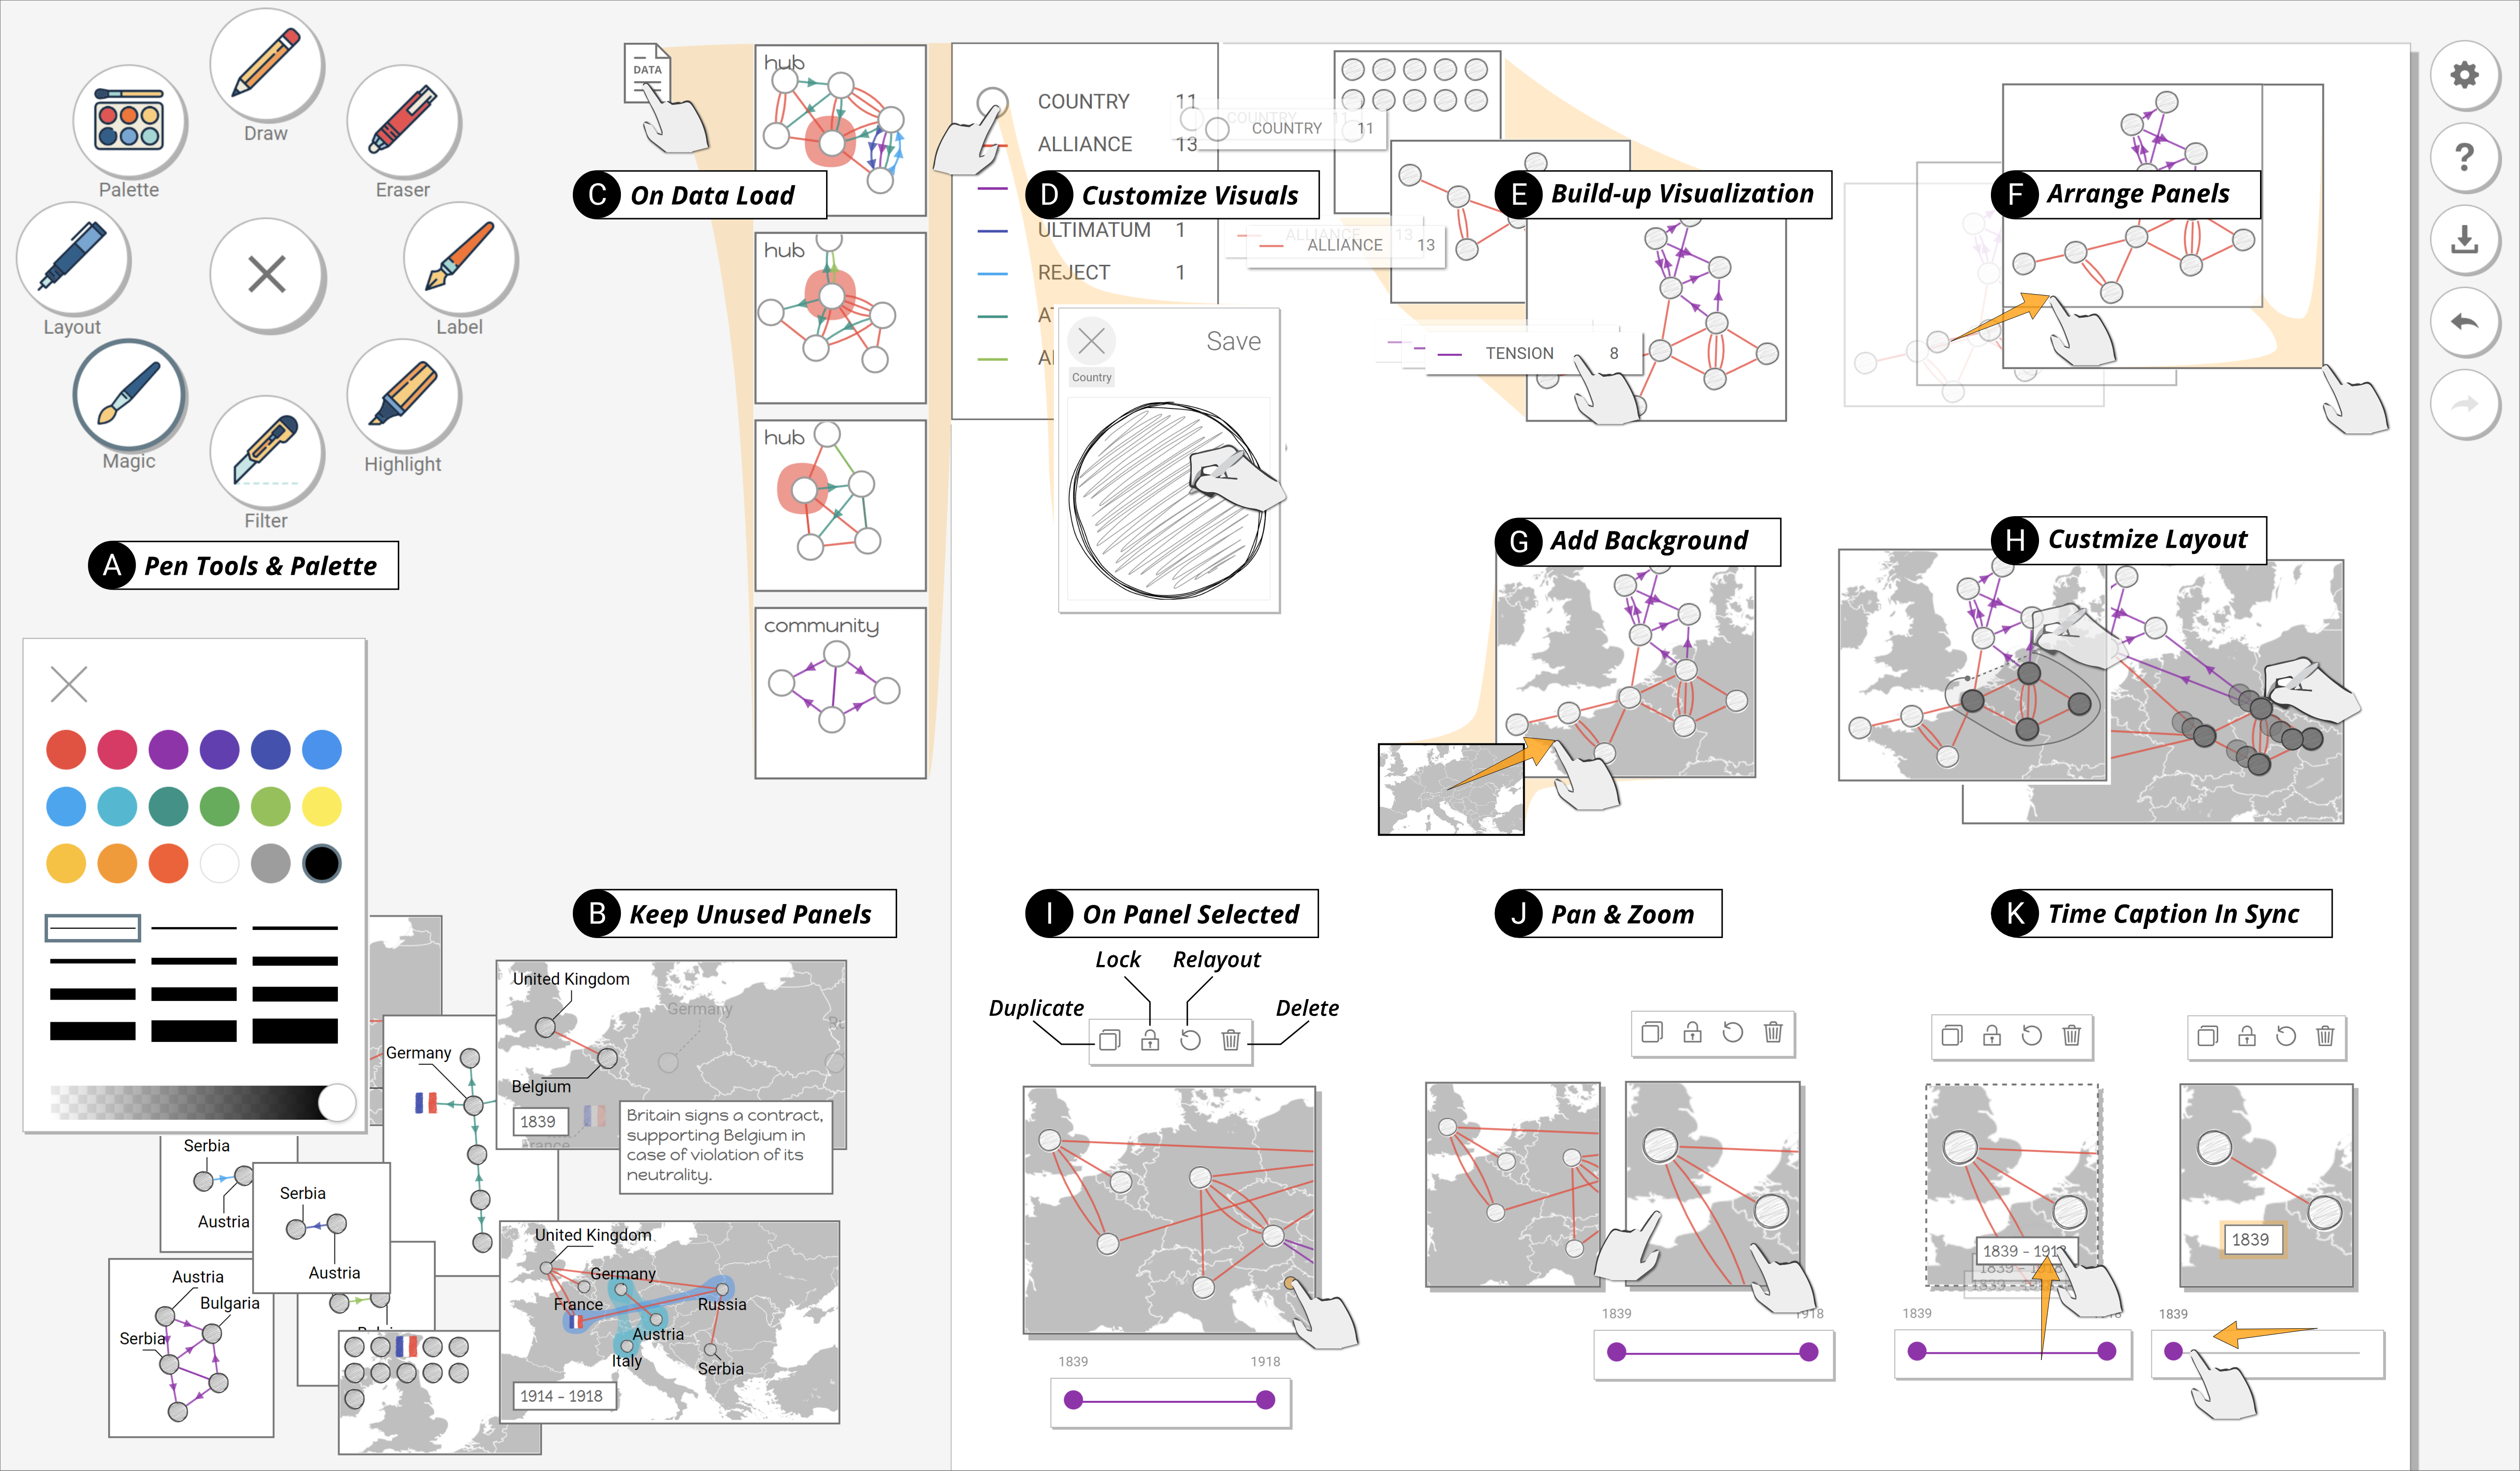
\includegraphics[width=1.0\textwidth]{figures/interface-overview.png} 
    \caption{\toolname{}'s interface: the pen can acquire different functions, such as labelling or filtering. The canvas area provides an infinite space for ideation and exploration, as well as a dedicated page area for presentation.}
    \vspace{-0.2cm}
    \label{fig:interface}
\end{figure*}

\section{Design Goals}
\label{sec:data_comics}


We conceive \toolname{} to accomplish three main goals.

\bpstart{D1. Support the creation of data \textit{comics}}
Data comics have unique characteristics and components~\cite{bach2017emerging,bachdesign}. They expose the story via a juxtaposed and sequenced panels, each containing one (or a few) insight(s). Getting the reader to focus on each insight requires that the author carefully crafts the view of each panel, such as zooming in on an important part of a network. However, identifying different characters of interest (e.g., nodes) and tracking them across panels requires that the author gives each a custom visual style to maintain consistency~\cite{qu2018keeping}. \toolname{} aims to support the crafting of panels and the expressive design of characters by direct manipulation using pen and touch, while ensuring consistency with data-driven propagation.

\bpstart{D2. Enable data-driven design}
Authoring tasks such as propagating visual designs across panels or creating transitions between panels are tedious and time-consuming. \toolname{} leverages the underlying data to automatically propagate visual designs of graphical elements and to generate textual labels and captions from data. \toolname{} also enables an author to generate transitional panels. For example, given two panels containing data at different times, \toolname{} can automatically create a series of panels representing the data at interim time points. 

\bpstart{D3. Support exploration and authoring activities}
Like any storytelling medium, the production of a comic is a creative and iterative process, often requiring the author to smoothly transition from reviewing the data and its patterns to styling them to craft a compelling story. \toolname{} facilitates the data exploration and review process by providing recommendations of interesting patterns in the data, such as a large cluster in the network, while enabling the rapid creation of visualizations using direct pen and touch manipulation. \toolname{} enables flexible workflows by providing a unique platform in which authors can review salient data aspects, rapidly generate and filter data visualizations, craft expressive visual design for data elements, compose a story by leveraging existing data comic templates, create a storyboard, or directly sequence and reorder panels. 
